\documentclass{report}

\usepackage{color}
\usepackage{amsmath}
\usepackage{graphicx}


\newcommand{\testcommand}{Hello}
\newcommand{\anothertestcommand}[2]{Welcome, #2! Mighty #1!!!}



\begin{document}
\begin{titlepage}
    \begin{center}
        \vspace*{1cm}
        
        \Large
         CSE300 ASSIGNMENT \\
         INTRODUCTION TO \LaTeX \\
         Introduction to Signal with Fourier Series \\
        \normalsize
        \vspace{1.5cm}
        Mohammed Latif Siddiq\\
        Student ID : 1505069
        
        \vfill
        
        \vspace{0.8cm}
        
        
\includegraphics[width=0.2\textwidth]{buetlogo.png}
        
        \Large
        Department of Computer Science and Engineering\\
       Bangladesh University of Engineering and Technology\\
      (BUET)\\
      Dhaka 1000\\
       \today
        
    \end{center}
\end{titlepage}

\newpage

\tableofcontents

\chapter{Signal}

\section{Introduction}

\subsection{Definition}
A signal is the term implies, is a set of \textbf{information} or \textbf{data}.It is a function of independent variables ( such as time,space \textit{etc}) that carry some information.\\
A signal is a physical quantity that \textbf{varies} with time, space or any other \textbf{independent variable} by which information can be conveyed.


\subsection{Example}
There is some example of signals: 

\begin{itemize}
    \item Voice signal
    \item Telephone or television signal
\end{itemize}


\subsection{Signal Representation}

In the following figure signal is represented in time domain:
\begin{figure}[h!]
    \centering
    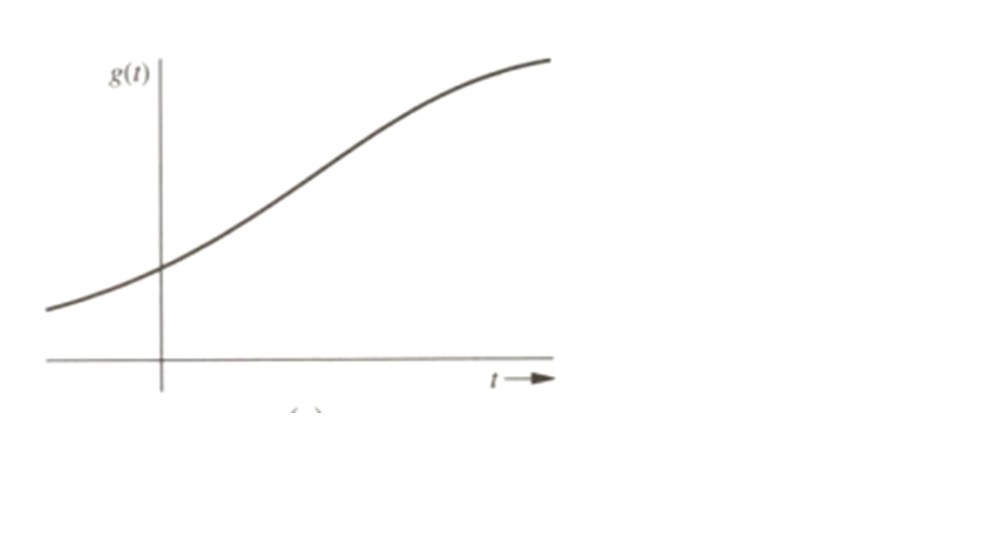
\includegraphics[width = 0.5\textwidth]{signal.png}
    \caption{Signal in time domain}
    \label{fig:signal}
\end{figure}


\section{Classification of Signals}
Signal can be classified based on two axes.

\begin{enumerate}
\item Based on continuity in time axis
      \begin{description}
        \item[Continuous time:] Speaking
    	\item[Discrete time:] Temperature Scale
      \end{description}

\item Based on continuity in amplitude axis
      \begin{description}
        \item[Continuous Amplitude:] Speaking
    	\item[Discrete Amplitude:] Road signal Light
      \end{description}

\end{enumerate}
Following figure describes signal based on time axis and amplitude axis
\begin{figure}[h!]
    \centering
    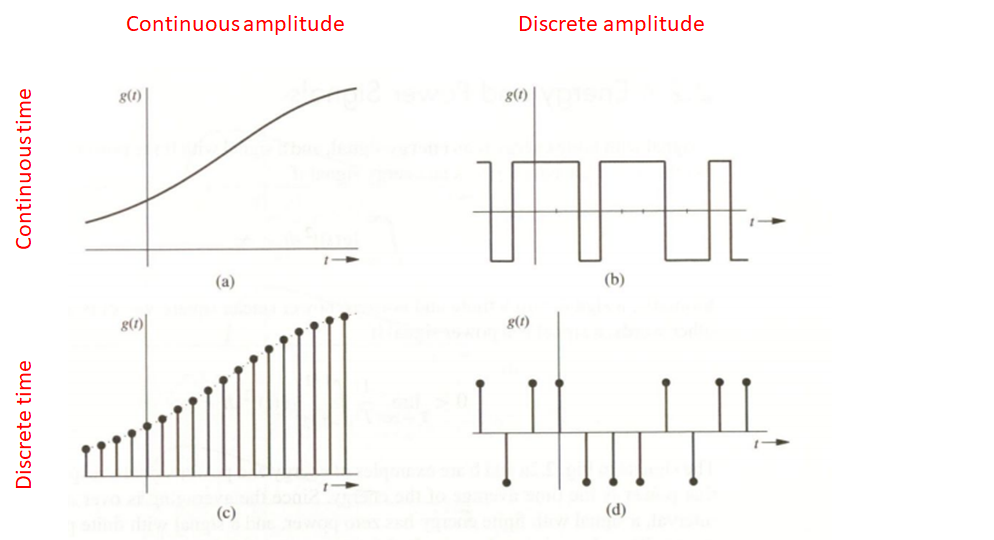
\includegraphics[width = .8\textwidth]{classsignal.png}
    \caption{Classification of Signal}
    \label{fig:classsignal}
\end{figure}

Signal also can be classified in following two types:
\begin{enumerate}
\item Analog Signal
\item Digital Signal
\end{enumerate}
Next section, we will discuss about this to type of signal.

\section{Analog and Digital Signal}

\subsection{Analog Signal}
An analog signal is any continuous signal for which the time varying feature (variable) of the signal is a representation of some other time varying quantity,\textbf{i.e.} , analogous to another time varying signal.It has continuous amplitude but time can be continuous or discrete.

In figure \ref{fig:signal}(a) and \ref{fig:signal}(c) is the examples of analog signal.
\subsection{Digital Signal}
A digital signal is a signal that is being used to represent data as a sequence of discrete values; at any given time it can only take on one of a finite number of values.This contrasts with an analog signal, which represents continuous values; at any given time it represents a real number within a continuous range of values.

In figure \ref{fig:signal}(b) and \ref{fig:signal}(d) is the examples of digital signal.

\subsection{Advantage of Digital Signal}
There are some advantages of digital signal over analog signal:
\begin{itemize}
\item Better noise immunity
\item Viability of regenerative repeaters
\item Hardware implementation is flexible with the use of integrated circuit, microprocessor etc.
\item Digital signal can be encoded for low error rate  and privacy 
\item Easier and efficient to multiplex digital signals
\item Digital signal storage is relatively easy and inexpensive
\item Decreasing cost of hardware with increasing capacity

\end{itemize}

\chapter{Fourier Series}
\section{Fourier Series}
In this chapter,we will discuss about \textbf{Fourier Series}.
\subsection{Fundamental Formulas}

Let $g_{T_0}$ denote a periodic signal with period $ T_{0} $ By using a Fourier series expansion of this signal, we are able to resolve it into an infinite sum of \textcolor{black}{sine} and \textcolor{black}{cosine} terms.
The expansion may be expressed in the \textit{trigonometric} form:

\begin{equation}
 g_{T_0}(t) = a_{0} + 2\sum_{n=1}^{\infty} [ a_n cos(2 \pi nf_{0}t) + b_n sin(2 \pi nf_{0}t) ]
 \label{eqn:furierfund}
\end{equation}
where $ f_{0} $ is the \textit{fundamental frequency}:
\begin{equation}
f_{0}=\frac{1}{T_{0}}
\label{eqn:fundfreq}
\end{equation}
The value of the co-efficient of the equation \ref{eqn:furierfund} can be determined by the following formulas:
\begin{equation}
a_{0} =  \frac{1}{T_{0}}\int_{T_{0}/2}^{-T_{0}/2} g_{T_0}(t) dt
\end{equation}
\begin{equation}
a_{n} =  \frac{1}{T_{0}}\int_{T_{0}/2}^{-T_{0}/2} g_{T_0}(t)cos(2 \pi nf_{0}t) dt
\end{equation}
\begin{equation}
b_{n} =  \frac{1}{T_{0}}\int_{T_{0}/2}^{-T_{0}/2} g_{T_0}(t)sin(2 \pi nf_{0}t) dt
\end{equation}
\subsection{Complex Form of Fourier Series}
The equation \ref{eqn:furierfund} can be expressed in the following  exponential form:
\begin{equation}
g_{T_0}(t) =\sum_{-\infty}^{\infty} c_{n} e^{\textit{j}2\pi nf_{0} t}
\end{equation}
where,
\begin{equation}
c_{n}= \frac{1}{T_{0}}\int_{T_{0}/2}^{-T_{0}/2} g_{T_0}(t)e^{-\textit{j}2\pi nf_{0} t} dt
\end{equation}

\end{document}
